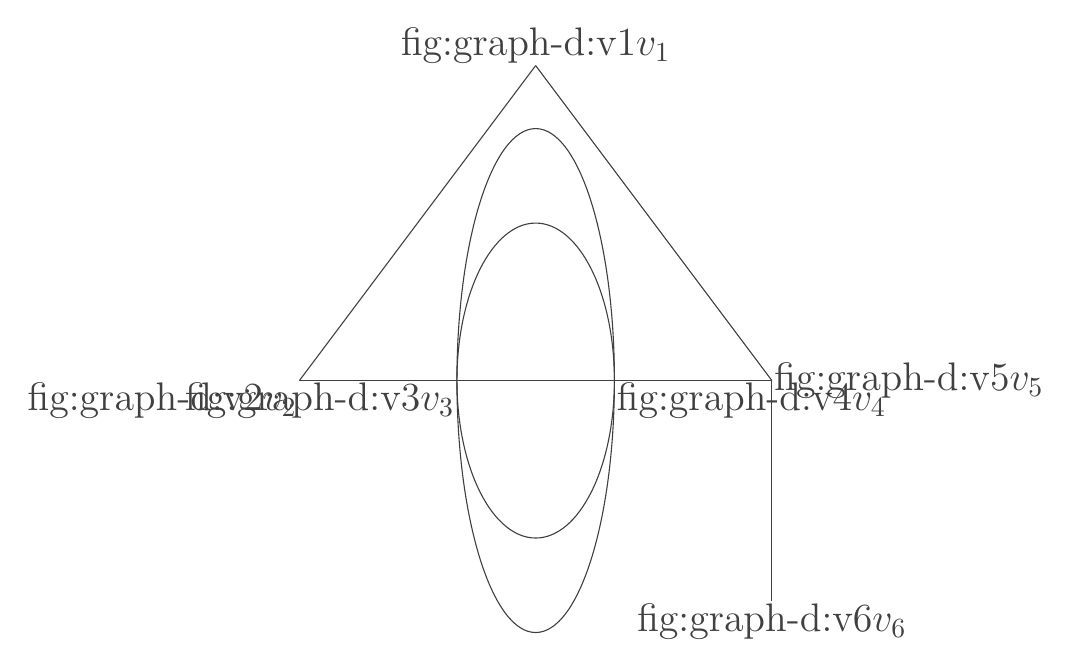
\begin{tikzpicture}[draw=darkgray, text=darkgray, align=center, xscale=1, yscale=2, scale=2]
    \tikzstyle{every node}=[inner sep=0pt];

    \node at ( 0.0, 1) (v1) [label=above:{\Large\hypertarget{fig:graph-d:v1}{$v_1$}}] {};
    \node at (-1.5, 0) (v2) [label=below left:{\Large\hypertarget{fig:graph-d:v2}{$v_2$}}] {};
    \node at (-0.5, 0) (v3) [label=below left:{\Large\hypertarget{fig:graph-d:v3}{$v_3$}}] {};
    \node at ( 0.0, 0) (vc) {};
    \node at ( 0.5, 0) (v4) [label=below right:{\Large\hypertarget{fig:graph-d:v4}{$v_4$}}] {};
    \node at ( 1.5, 0) (v5) [label=right:{\Large\hypertarget{fig:graph-d:v5}{$v_5$}}] {};
    \node at ( 1.5, -0.7) (v6) [label=below:{\Large\hypertarget{fig:graph-d:v6}{$v_6$}}] {};

    \draw (v1.center)
        edge (v2.center);
    \draw (v3.center)
        edge (v2.center)
        edge (v4.center);
    \draw (v5.center)
        edge (v1.center)
        edge (v4.center)
        edge (v6.center);
    \draw (vc.center) ellipse (0.5 and 0.8);
    \draw (vc.center) ellipse (0.5 and 0.5);
\end{tikzpicture}
